% ============================================================================
% *** VERSION 2 *** — do NOT edit octopus_behaviour_pipeline.tex from here.
% v1 (octopus_behaviour_pipeline.tex) is frozen as the last known-good 7-page draft.
% v2 adds: (a) the dataset-gap motivation, (b) a quantified "foundation models out of
% the box" passage (OWLv2 231/232, GD+SAM2 bleed numbers), (c) related-work positioning
% against HideAndSeg (arXiv 2511.04426) incl. the evaluation-protocol difference.
% DRAFT — OCEANS 2026 companion paper (behaviour-profiling pipeline).
% Sibling paper: conference_101719.tex (protest-behavior -> lighting).
% All reported numbers trace to PAPER_NOTES.md / data/benchmarks.json (frozen suite;
% see BENCHMARKS.md). Table \ref{tab:benchmarks} is auto-generated by src/benchmarks.py
% into assets/benchmarks_table.tex — do not hand-edit it here.
% Open before submission:
%   - finalise author list / affiliations (placeholder below, mirrors the consortium)
%   - \cite{hideandseg} author list filled from the arXiv record (de Aguiar, Andrade, Santos,
%     Gois; all Universidade Federal do ABC, Brazil), verified 2026-08-19.
% v2 additions and their provenance:
%   - Table \ref{tab:teacher} (teacher vs student on human masks) = PAPER_NOTES R19 /
%     data/teacher_vs_human_masks.json, measured 2026-08-20 by src/eval_teacher_masks.py.
%     This one IS a new measurement. The frozen set is IMPORTED from benchmarks.py, and the
%     student reproduced its published 0.6415 exactly, which validates the harness.
%     Cite it as the PER-FRAME teacher only. The propagated labels the student actually
%     trained on are better, so 0.374 is a LOWER bound on teacher quality -- do not write it
%     as "the teacher's mask quality". The propagated-label arm needs 122x40 = 4,880
%     GroundingDINO calls (~3.4 h) and has NOT been run.
%     Also: 5 clusters makes the CI wide -- claim the ordering, not the magnitude.
%   - Sec.III-A "What the probe adds over CLIP alone" = PAPER_NOTES R22 /
%     data/zeroshot_vs_probe.json, measured 2026-08-20 by src/eval_zeroshot_vs_probe.py.
%     NEW measurement. Set = EMPTY-V2's 120 HUMAN-labelled frames / 60 videos, sampled at uniform
%     random timestamps over WHOLE source videos, so it is detector-INDEPENDENT, and leak-free
%     (empty_negatives.py excludes thin768's 142 training videos AND the CLIP detector's sessions).
%     Both arms share the frozen CLIP ViT-B/32 backbone + letterbox, so the delta isolates the probe.
%     Zero-shot got a deliberately generous 5+5 prompt ENSEMBLE (prompts stored in the json) so it is
%     not a strawman. DO NOT quote the probe's 0.745 as comparable to the 96.8% accuracy -- different
%     metric AND a harder, unbiased set. Only 23 positives: claim the ordering, never the magnitude.
%   - HideAndSeg related-work numbers = PAPER_NOTES R20, read from the arXiv HTML full text
%     (2511.04426v1) on 2026-08-20, verified against their own Tables 1-2:
%       * DICE/IoU identical to 4dp incl. SD across 5/10/20 annotated frames (0.9677+-0.0191 /
%         0.9383+-0.0349), and the "+ additional frame" rows move them by EXACTLY zero.
%       * "manual segmentation on the initial frame of all videos"; tables are labelled
%         "Supervised Metrics (first frame)".
%       * 35% presence pre-filter = 366,514 usable of 564,755 raw frames.
%       * ~249M deployed = YOLOv11-l (25.3M) + SAM2.1-hiera-large (224M); no runtime reported.
%     DO NOT write "~17 test frames" (an earlier R18 slip): they split by FRAMES (test 36,079)
%     and never report the test VIDEO count. If a count is needed, say it is unreported.
%     Their field coverage genuinely exceeds ours (3 sites / 7 expeditions, wild, multi-animal
%     vs our single individual) -- that concession is deliberate, keep it.
% Everything below was pre-existing at the time v2 was forked (nothing new was run for these):
%   - OWLv2 231/232 at thr 0.10 + the 166/232 human outcome: AGENTS.md "Hard-negative mining"
%     (data/hard_negatives/_detector_verify.json, review_decisions.csv). Logged there, not yet
%     mirrored into PAPER_NOTES.md's ledger - mirror it when PAPER_NOTES is next editable.
%   - Phase-0 teacher bleed 11.8->6.5 (IR) / 15.5->5.8 (colour), seed conf ~0.50 vs 0.74-0.89:
%     PAPER_NOTES R3 + AGENTS.md "Phase 0 DONE".
%   - IR 13% clip acceptance (87 of 653): src/SEGMENTATION_LOG.md "IR auto-labeling - FAILED".
%   - zero-shot CLIP detection invalidated 2026-06-13: AGENTS.md "Persistent memory" note.
% Presence numbers (Table \ref{tab:presence}) = PAPER_NOTES R14 / data/presence_human_verified.json:
%   negatives are HUMAN-verified (EMPTY-V2 120/120, reflection 42/42), so R9/R10/R13 are now
%   citable. Cite ONLY the human-verified figures; the earlier AI-labelled versions (0.9170,
%   0.9214, 0.9315, 0.8053, +0.1263) were optimistic on both sets and must never be used.
%   Not cited, deliberately: the combined rank-product gate (R10) has no human-verified
%   re-measurement; the withdrawn "failure mode is backwards" claim (R9 CORRECTION).
% Label reliability = PAPER_NOTES R15 / data/vlm_reliability_stats.json (VLM-250, 250 clips /
%   140 videos, disjoint frame set). It measures CONSISTENCY, never accuracy.
% Kinematics numbers = PAPER_NOTES R12 (data/kinematics_stats.json, 146 clips / 66 videos,
% video-level). Fig. 4 is generated from the same loader (src/kinematics_stats.collect).
% Cut for space (logged in PAPER_NOTES R8-FINAL, still true): the fusion threshold sweep
% also showed the shipped binarisation threshold is mildly suboptimal (+0.0137 IoU at 0.80,
% not applied - the skeleton stage consumes these masks and needs its own SKEL-50 A/B).
% ============================================================================
\documentclass[conference]{IEEEtran}
\IEEEoverridecommandlockouts
\usepackage{cite}
\usepackage{amsmath,amssymb,amsfonts}
\usepackage{algorithmic}
\usepackage{graphicx}
\usepackage{textcomp}
\usepackage{xcolor}
\usepackage{enumitem}
\usepackage{booktabs}
% float placement: let pages carry more float area (avoids half-empty float pages)
\renewcommand{\topfraction}{0.92}
\renewcommand{\bottomfraction}{0.7}
\renewcommand{\textfraction}{0.06}
\renewcommand{\floatpagefraction}{0.85}
\def\BibTeX{{\rm B\kern-.05em{\sc i\kern-.025em b}\kern-.08em
    T\kern-.1667em\lower.7ex\hbox{E}\kern-.125emX}}
\begin{document}

\title{From Footage to Ethogram: An Automated Vision--Language Pipeline for
Quantifying Behaviour and Affective State of a Captive Octopus}

% TODO: confirm/finalise author list and ordering with the consortium.
\author{
\IEEEauthorblockN{
Siddharth Raj\IEEEauthorrefmark{1},
Harald Burgsteiner\IEEEauthorrefmark{2},
Wolfgang Slany\IEEEauthorrefmark{3}
}
\IEEEauthorblockA{\IEEEauthorrefmark{1}
Research and Development, Arishna IoT Solutions, Bangalore, India}
\IEEEauthorblockA{\IEEEauthorrefmark{2}
Institute for Digital Media Education, University of Teacher Education Styria, Graz, Austria}
\IEEEauthorblockA{\IEEEauthorrefmark{3}
Institute of Software Engineering and Artificial Intelligence, Graz University of Technology, Graz, Austria}
}
\maketitle

\begin{abstract}
Continuous camera monitoring of captive marine animals produces far more video
than caretakers can review, yet most of it is used only reactively. We present
an automated vision--language pipeline that converts continuous multi-camera
aquarium footage of a single \emph{Octopus vulgaris} into a quantified
behavioural and affective-state time-series. It detects when the
animal is visible (a frozen CLIP encoder with a lightweight probe under
aspect-preserving preprocessing), extracts short behaviour clips gated on
visibility and motion, and re-prompts a large vision--language model for a
structured behavioural record per clip (behaviour class, posture, activity,
location, context and body colour). Aggregating $3{,}083$ analysed clips yields
an interpretable activity budget, an exposure-normalised circadian profile with a
late-afternoon activity peak, and a clear stimulus response in which human
presence nearly doubles movement and raises a transparent arousal index. To make
the system self-hosting we distil the teacher into small local models: a
captioning student (Qwen3-VL-2B~\cite{qwenvl}, QLoRA) running 4-bit on a laptop,
and a single-class mask model auto-labelled by GroundingDINO and SAM2 and
anchored by human-verified masks. On a
leak-free human-labelled test (122 frames from five held-out source videos) that
model reaches $0.64$ mean / $0.72$ median IoU with $1.1\%$ body-area error, and
its mask area doubles as the pipeline's presence gate---AUC $0.91$ against
human-verified empty frames from $52$ recordings, and indistinguishably $0.91$
against tank-glass reflections, retiring our assumption that reflections were
the dominant failure mode---which works only because the student is trained
with empty-mask negatives. On top of
the masks we extract an \emph{anatomical skeleton}---mantle, head and up to eight
arm splines---scored on a frozen benchmark by arm-tip F1 against protrusions of
the human mask ($0.54$), a metric adopted only after ``arms per frame'' proved
gameable and the replacement's own ground truth proved wrong. Its
occlusion-honest arm kinematics independently separate the VLM-derived behaviour
classes on $146$ clips from $66$ source videos, aggregated to one value per
(video, class) before testing (median arm-tip speed $53$\,px\,s$^{-1}$ resting
vs.\ $141$ reaching out of water; Kruskal--Wallis
$p{=}3.5\!\times\!10^{-6}$, $\varepsilon^2{=}0.22$, and still significant in
scale-invariant body-lengths per second): a cross-validation of two signal paths
that share no components. We frame results as arousal and behavioural state
rather than emotion, measure the reliability of the very labels the analysis
groups by (Cohen's $\kappa{=}0.55$ under a disjoint frame sample---moderate, and
a bound on every aggregate here), report the limitations and the measured
negative results honestly, and position the work as the profiling layer
complementary to real-time single-behaviour response systems.
\end{abstract}

\begin{IEEEkeywords}
Computer Vision; Vision--Language Models; Behaviour Analysis; Marine Animal
Welfare; Model Distillation; Edge AI; Cephalopods
\end{IEEEkeywords}

\section{Introduction}
Aquarium and controlled-habitat monitoring increasingly relies on continuous
camera coverage, but the resulting video vastly exceeds what caretakers can
review. Most footage is therefore consulted only reactively, and the record of
an animal's day-to-day behaviour is left unquantified. For welfare-oriented
husbandry the more valuable question is longitudinal: \emph{how does this animal
spend its time, and how does it respond to its environment?}

Octopuses make this both important and hard. They are highly intelligent,
behaviourally complex invertebrates whose welfare is a growing concern, yet their
non-rigid bodies, rapid posture changes, active camouflage, frequent denning, and
the reflections and floating debris of tank environments defeat naive visual
monitoring~\cite{disc_o}. A companion line of work from our consortium targets a
single, actionable behaviour---a ``protest'' limb gesture used to request tank
lighting---and actuates the lights; that system is reactive and
behaviour-specific by design.

This paper addresses the complementary problem: \emph{understanding the whole
behavioural repertoire over time}. We present an automated pipeline that turns
continuous multi-camera footage of one captive \emph{O.\ vulgaris} (``Nity'')
into a structured behavioural and affective-state time-series, together with the
small local models needed to run it cheaply and offline.

One constraint shapes the entire design. There is no large-scale, publicly
available annotated dataset for octopus segmentation or detection to train
on---an absence independently reported by concurrent work on octopus
segmentation in natural habitats, which cites ``the absence of large-scale,
publicly available, annotated video datasets for octopus segmentation, which
prevents standard supervised fine-tuning and evaluation''~\cite{hideandseg}. So
supervised training on an existing corpus was never an option, and every label
in this pipeline has to be manufactured: by foundation-model teachers run
offline over our own footage, by a human wherever the measurement depends on it,
or not at all. That is why the architecture is teacher$\rightarrow$student
distillation rather than fine-tuning, and why so much of what follows is about
verifying labels we generated ourselves. Our contributions are:
\begin{enumerate}[leftmargin=*, itemsep=1pt, topsep=2pt]
\item An end-to-end pipeline from raw footage to a per-clip \emph{structured
behavioural record}, using a large vision--language model (VLM) as a
zero-shot behavioural annotator with snap-to-list validation.
\item An aggregate behavioural analysis over a nine-day observation window
($3{,}083$ present clips, seven recording days): an interpretable activity
budget, an exposure-normalised circadian profile, and a quantified stimulus
response, framed as arousal / behavioural state.
\item Teacher$\rightarrow$student distillation into deployable local models---a
4-bit captioning student that runs on a laptop, and a single-class octopus
segmentation model auto-labelled by GroundingDINO$+$SAM2, anchored by
human-verified masks, and evaluated leak-free on a held-out human-labelled test
($0.64$ mean / $0.72$ median IoU, $1.1\%$ body-area error --- one model, one
test set, with the split re-derived to prove the holdout was never trained on).
\item An anatomical skeleton and kinematics layer on the masks: per-frame
mantle/head/arm graphs scored by arm-tip F1 on a frozen benchmark, with the
arm-selection gates reported as an explicit precision--recall frontier rather
than a single tuned point; occlusion-honest tracking; and per-arm kinematics
that separate the VLM behaviour classes with video-level statistics on $146$
clips from $66$ recordings---a cross-validation of two unrelated signal paths.
\item A frozen benchmark suite (segmentation, skeleton, tracking; one runner,
tagged results, video-level splits) and an honest account of the methodology
around it, including measured negative results: a train--test leakage we caught
and corrected, a headline metric retired because a genuine improvement made it
worse, a metric ground truth we had to validate and fix, a null result retiring
our own assumption about the pipeline's dominant failure mode, and several
plausible improvements that failed under the fixed benchmark.
\end{enumerate}

\section{Related Work}
\textbf{Cephalopod behaviour and welfare.} Interest in octopus cognition and
welfare has grown alongside their inclusion in animal-welfare frameworks. Prior
consortium work introduced a framework for decoding inter-species communication
with octopodes and a real-time detector for a light-request behaviour that
actuates the habitat~\cite{disc_o}; our work is the profiling counterpart to
that response system.

\textbf{Foundation models as annotators.} General-purpose VLMs describe and
classify images zero-shot, and open-vocabulary detectors and promptable
segmenters (GroundingDINO~\cite{groundingdino}, SAM/SAM2~\cite{sam2}) label
without task-specific supervision. We use these as \emph{teachers}, distilling
their labels into small students~\cite{lora}. CLIP~\cite{clip} provides the
frozen features for our presence detector; the deployed segmenter uses an
LR-ASPP/MobileNetV3 head~\cite{mobilenetv3}. Off the shelf, however, these
models were not usable as detectors on our footage; Sec.~\ref{sec:distill}
quantifies where they failed.

\textbf{Octopus segmentation in the field.} The closest work to ours is
HideAndSeg~\cite{hideandseg}, a concurrent annotation-light segmentation
pipeline: a human annotates initial frames to prompt SAM2, the resulting masks
train a YOLOv11 detector, and that detector then auto-prompts SAM2 over the
remaining footage. On $148$ videos of juvenile \emph{Octopus insularis}
($366{,}514$ usable frames) recorded at three Brazilian coastal sites, it reports
DICE $0.9677$ and IoU $0.9383$. Their central insight---re-detecting per frame so
that a contaminated propagation track can recover---is correct, and our
seed-confidence gate serves the same purpose. Their field coverage also exceeds
ours: wild animals at three sites across seven expeditions, against our single
individual in one tank (Sec.~\ref{sec:limits}).

Those figures are not comparable with the $0.641$ IoU we report, and we would
rather say so than let the contrast be drawn for us. (i)~\emph{The reference
differs.} Their ground truth is manual segmentation of the initial frame of each
video---essentially the frame used to prompt SAM2---while ours is $122$
human-drawn masks sampled across five source videos held out of \emph{all}
training. Their own tables show the consequence: DICE and IoU are identical to
four decimal places, standard deviations included, whether the auto-prompting
detector is trained on $5$, $10$ or $20$ annotated frames, and adding a second
annotation frame moves them by exactly zero---the supervised metric is
insensitive to the propagation it is meant to assess. (ii)~\emph{The imaging
conditions differ}: natural-habitat colour video against dim aquarium footage
with infrared cameras, tank-glass reflections and clutter. (iii)~\emph{The
subject differs}: juvenile \emph{O.\ insularis} against an adult
\emph{O.\ vulgaris}. (iv)~\emph{Presence is given rather than inferred}: frames
without a visible octopus are removed before their pipeline runs ($35\%$ of the
raw footage), whereas deciding presence is precisely what our gate must do
(Table~\ref{tab:presence}). (v)~\emph{The deployment target differs}, which is
our actual distinction: they run YOLOv11-l plus SAM2-hiera-large,
$\approx\!249$\,M parameters, at inference and report no runtime, whereas we
distil to a $3.2$\,M-parameter student---$\approx\!78\times$ smaller---that runs
locally with no GPU and no API.

Read on a single axis, though, the numbers agree rather than conflict: mask
quality tracks how much prompting is assumed at inference. Their $0.938$ is
box-prompted; our teacher reaches $0.726$ on the frames where it clears its own
seed-confidence gate (Table~\ref{tab:teacher}); our student reaches $0.641$ with
no prompt at all. The open problem is therefore not prompted mask quality but
unprompted, dense, deployable coverage---which is what distillation supplies and
what a behavioural layer running unattended requires. The two lines are
complementary rather than competing: they solve automated \emph{prompting} of a
large model in the field, we solve \emph{distillation to a deployable model} and
the behavioural layer built on it. That both projects had to manufacture their
own labels is the same finding reported twice.

\section{System and Methods}
The tank is observed by a multi-camera rig (6 IP cameras, 4K, infrared and colour
night vision) with a manually selected region of interest around the den per
camera; the same installation supports the companion response system.

% FIGURE: pipeline diagram (detection -> extraction -> structured extraction -> distillation).
% generate from src/ (draw in draw.io / tikz). Placeholder path below.
\begin{figure}[t]
    \centering
    
\includegraphics[width=0.48\textwidth]{assets/pipeline_behaviour.pdf}
    \caption{Footage-to-ethogram pipeline (the four stages of Sec.~III):
    visibility detection $\rightarrow$ clip extraction $\rightarrow$ VLM
    structured behavioural extraction $\rightarrow$ distillation into local
    caption and segmentation students.}
    \label{fig:pipeline}
\end{figure}

\subsection{Visibility Detection}
\label{sec:detect}
A frozen CLIP ViT-B/32 encoder feeds a small multi-layer-perceptron probe
(512$\rightarrow$256$\rightarrow$64$\rightarrow$2) classifying
\emph{octopus-visible} vs.\ \emph{hidden}. The single most important design
choice was preprocessing: CLIP's default centre-crop discards $33$--$44\%$ of a
16:9 frame, and \emph{aspect-ratio mismatch}---not backbone capacity---was the
root cause of poor field performance. Aspect-preserving letterbox padding plus
$\sim$1.7k mined reflection/infrared-noise hard negatives gave a probe reaching
$96.8\%$ on our internal detection test set.

\textbf{What the probe adds over CLIP alone.} That $96.8\%$ is an internal-split
accuracy with no baseline, so it cannot attribute performance to the probe rather
than the backbone. On $120$ human-labelled frames from $60$ recordings, drawn at
uniform random timestamps over whole source videos---so nothing was selected by
the model under test---and excluding every session used in training, prompting
the same frozen encoder instead of the probe (a five-plus-five octopus/empty
prompt ensemble) scores AUC $0.450$, CI95 $[0.259,0.643]$: chance, with a median
score \emph{higher} on empty frames than on frames containing the animal. The
probe reaches $0.745$ $[0.564,0.890]$, a paired $\Delta$AUC of $+0.295$
$[+0.069,+0.528]$, cluster-bootstrapped by source video and excluding zero. As
both arms share backbone and preprocessing, the gap isolates the probe: CLIP
supplies features, and the discriminative ability is essentially all supervised.
Only $23$ frames contain the animal, so we claim the ordering, not the magnitude.

\subsection{Clip Extraction}
Per second of source video we compute the probe's visibility probability and an
absolute changed-pixel motion fraction (with the burned-in timestamp region
masked so the ticking clock is not counted as motion), and keep a
non-overlapping $20\,\mathrm{s}$ window when the octopus is visible for a
majority of it and mean motion exceeds a threshold. The \emph{absolute} fraction
is deliberate: per-video normalised motion promotes static scenes (a flickering
lamp) to ``motion''.

\subsection{Structured Behavioural Extraction}
Rather than treating a caption as the end product, we treat it as one field of a
\emph{structured behavioural record}. Per clip we select the clearest frames
(contrast-enhanced for the dim infrared footage, scored by the visibility probe)
and prompt a large VLM (Qwen3-VL-235B~\cite{qwenvl}, via API) for a JSON record:
\{present, behaviour (7-class ethogram), posture, activity level, location,
context, body colour, colour/texture change, confidence\}. Each
field is validated by snapping to an allowed value list; colour fields are gated
per clip, so infrared/greyscale clips (detected by low BGR channel divergence)
are told to leave colour \emph{uncertain}. The run over $3{,}205$ clips cost
$\approx\$2.22$ ($\sim\$0.0006$/clip). One field of the schema is dead and we
report it as such: \emph{colour/texture change} was never once asserted across
the $99$ colour clips of the reliability sample, so it carries no signal and is
a candidate for redesign. The visibility probe is the weaker of our two presence
signals; Sec.~\ref{sec:models} measures it head-to-head against the mask-area
gate rather than by anecdote.

\subsection{Distillation to Local Models}
\label{sec:distill}
The expensive foundation models are used only as \emph{offline teachers};
nothing large is deployed. Their outputs become training data for small
students, so the running system is self-hosting and needs no GPU server or paid
API. We apply the recipe twice---VLM captions into a compact captioning model,
GroundingDINO$+$SAM2 masks into a single-class segmentation model
(Sec.~\ref{sec:models})---each kept as small as the task allows so continuous
in-situ inference is feasible on commodity hardware.

\textbf{Why distil rather than prompt.} Distillation is not only a cost
argument: we measured the off-the-shelf alternatives on this footage and none of
them worked as a detector. Asked to verify $232$ mined hard-negative frames, an
open-vocabulary detector (OWLv2~\cite{owlv2}) reported an octopus in $231$ of
them at a $0.10$ threshold. Human review of the same frames found that $166$
genuinely contained the animal and $66$ did not. Its scores are not
uninformative---they rank the two classes at AUC $0.759$---but the
distributions overlap so heavily that no threshold yields a usable filter: at
its own best operating point ($0.23$, Youden $J=0.378$) it still passes $30$\%
of the frames we wanted removed while discarding $32$\% of the real animals,
and any threshold retaining $\geq\!95$\% of the animals passes $70$\% of the
negatives. A weak ranking signal with no viable operating point is not a
detector. Zero-shot CLIP scoring for
presence was likewise abandoned as unreliable; what works is a \emph{trained}
probe on frozen CLIP features (Sec.~\ref{sec:detect}), and even that is the
weaker of our two presence signals. The promptable segmentation teacher is
usable, but only when gated by seed confidence and propagated through time---
prompted per frame it is beaten by our $3.2$\,M-parameter student on the same
human masks (Table~\ref{tab:teacher})---and it fails outright on one of our
cameras (Sec.~\ref{sec:models}). Read together,
these say the same thing: the foundation models here are \emph{gated,
temporally propagated offline annotators}, not drop-in detectors---which is
exactly the case for distilling them into a student rather than prompting them
at inference time.

\subsection{Diverse-Footage Harvesting}
\label{sec:harvest}
Early models were trained on footage from a single week, the binding
generalisation limit. We therefore built a streaming harvester that crawls the
archive and \emph{probes} a handful of frames per candidate video before
committing to a full scan, skipping empty ``den'' videos cheaply. Because the
server imposes a low aggregate bandwidth cap (measured $\sim$5\,MB/s, parallel
connections yielding only $1.6\times$), it runs as a single CPU worker that
streams rather than bulk-downloads, keeping a coverage ledger so skipped footage
can be revisited---expanding coverage from $7$ to $>\!100$ distinct days.

\subsection{Evaluation Protocol: a Frozen Benchmark Suite}
\label{sec:bench}
A pipeline this long makes it easy to accumulate numbers each measured on a
slightly different set, so we froze three benchmarks behind a single runner
writing tagged results, making every improvement claim a before/after on the
same data. \emph{SEG-TEST}: $122$ human-labelled mask frames plus $19$
empty-mask negatives, from five source videos excluded from \emph{every}
training source; mask IoU, body-area error, presence AUC. \emph{SKEL-50}: $50$
frozen frames over $20$ source videos, each with image, human mask and model
mask; arm-tip F1. \emph{TRACK-10}: $10$ frozen clips spanning all six behaviour
classes, three cameras and three dates; teleport rate, occluded fraction,
coverage. Two rules hold throughout: splits are by \emph{source video}, never by
frame---frames from one recording are near-duplicates and we shipped that bug
once (Sec.~\ref{sec:models})---and the frozen lists are never regenerated to
suit a result (Table~\ref{tab:benchmarks}).

We also verify ``held out'' rather than assert it. All five SEG-TEST videos
appear in the deployed model's \emph{dataset} manifest, which lists every
labelled pair, but a forced-holdout flag keeps them out of training: re-deriving
the split from the manifest, source filter and seeded shuffle reproduces the
logged partition exactly ($3{,}450$ train / $1{,}693$ validation frames), with
no holdout video in training. The audit also exposed---and we fixed---a logging
bug printing wrong video counts for a correct split, which is what a leak looks
like at a glance.

% auto-generated by src/benchmarks.py — do not hand-edit
% regenerate without re-running the models: src/benchmarks.py --latex-from <tag>
\begin{table}[t]
\caption{Frozen benchmark suite, deployed configuration (octo\_seg\_thin768\_lraspp.pt). All splits are by
SOURCE VIDEO; the segmentation test videos are excluded from every training source.
Mask IoU comes from the same model and test set as the presence row, but that row's
19 negatives come from only two recordings; it is retained for continuity and is
superseded by the multi-recording human-verified negative sets reported in the text.
Tip-F1 scores arm recovery against the human mask's protrusions, so both missed and
spurious arms are penalised; arm count is descriptive only.}
\label{tab:benchmarks}
\centering
\small
\begin{tabular}{@{}lc@{}}
\toprule
Metric & Value \\
\midrule
\multicolumn{2}{@{}l}{\textbf{SEG-TEST} --- 122 human-mask frames, 5 held-out videos} \\
\quad mask IoU (mean / median) & 0.641 / 0.719 \\
\quad body-area error & 1.05\% \\
\quad presence AUC (vs 19 empty, 2 recordings) & 0.794 \\
\midrule
\multicolumn{2}{@{}l}{\textbf{SKEL-50} --- 50 frozen frames} \\
\quad arm-tip F1 & 0.539 \\
\quad tip precision / recall & 0.722 / 0.502 \\
\quad arms per frame (descriptive) & 3.68 \\
\bottomrule
\end{tabular}
\end{table}


\section{Behavioural and Affective-State Analysis}
Aggregating the $3{,}083$ present clips (joined to absolute clock time) yields an
interpretable behavioural profile. These clips come from \emph{seven recording
days spanning nine calendar days} (20--28 February 2026), so the profile below
characterises one observation window rather than a season: the circadian curve in
particular is an average over seven days, and we make no claim about seasonal or
long-term drift. Extending this analysis across the harvested $\sim\!209$-day
corpus is the immediate next step (Sec.~\ref{sec:limits}). We report \textbf{arousal and behavioural
state}, not emotion; the transparent arousal index is
$0.6\cdot\mathrm{activity} + 0.4\cdot\mathrm{posture\text{-}spread}$, with static
body colour a secondary channel on colour cameras only.

% FIGURE: activity budget + circadian + stimulus-response (from data/behaviour_dashboard.html)
\begin{figure}[t]
    \centering
    
\includegraphics[width=0.48\textwidth]{assets/behaviour_findings.pdf}
    \caption{Aggregate behaviour from the structured records: (a) activity
    budget; (b) exposure-normalised circadian visible-activity rate; (c) motion
    and arousal with vs.\ without human presence.}
    \label{fig:findings}
\end{figure}

\textbf{Activity budget.} Exploration/manipulation $41\%$, resting $33\%$,
human/enrichment interaction $14\%$, reaching out of water $9\%$, crawling
$2\%$, swimming/jetting $1\%$ (Fig.~\ref{fig:findings}a).

\textbf{Circadian structure.} Normalising present-clip counts by all extracted
windows per hour (an exposure correction) reveals a strong diel pattern: visible
activity is $\sim$1--5\% overnight and rises to a $\sim$45\% peak at 17:00 with a
13:00--19:00 plateau, plus a dawn bump at 05:00--06:00.

\textbf{Stimulus response.} With vs.\ without a human present, mean motion nearly
doubles ($0.045\rightarrow0.095$) and the arousal index rises
($0.46\rightarrow0.68$). On colour cameras the dark red-brown body colour is most
common at baseline ($\sim$16\%) and less so during human interaction ($\sim$6\%).
We regard such \emph{contrasts} as the robust findings; absolute levels depend on
the upstream presence gate and will shift as the detector improves.

\section{Local Models}
\label{sec:models}
\subsection{Captioning Student}
We distil the teacher's one-sentence descriptions into Qwen3-VL-2B~\cite{qwenvl}
using QLoRA (rank 16). On a $50$-clip held-out split, embedding similarity to
the teacher improves from $0.702$ (base) to $0.834$ and ROUGE-L from $0.269$ to
$0.455$. Quantised to 4-bit with MLX, the student is $\sim$1.7\,GB and captions
a clip in $\sim$3\,s on a 16\,GB laptop with no GPU.

\subsection{Segmentation Student}
Following Sec.~\ref{sec:distill} we target the \emph{smallest} model that yields
usable masks: one foreground class at low resolution, with GroundingDINO (box)
$+$ SAM2 (mask) as an offline auto-labeller, never deployed. The most-confident
frame seeds SAM2 video propagation, and largest-blob plus area-continuity
cleanup remove transient errors.

That recipe is a correction, not a refinement. Prompting the teacher
independently per frame over-segments in two systematic directions, both
measurable: on the infrared camera SAM2 attaches to bright metal tools, and
seeding a single propagated track cuts mask area from $11.8\%$ to $6.5\%$ of the
frame; on colour cameras the mask escapes the loosely fitted box into the
background, $15.5\%$ to $5.8\%$. Clips already clean show no regression. Seed
confidence supplies the rest: on the tank-glass reflection camera
GroundingDINO's best frame peaks at $\approx\!0.50$ against $0.74$--$0.89$ on
real animals, so the camera is rejected wholesale rather than quietly
mislabelled. The limit of the recipe is worth stating with its success, because
it is the same mechanism: temporal propagation removes errors that are
\emph{transient} across a clip, and cannot touch errors that are
\emph{consistent}---a reflection is present in every frame---which is why
confidence gating is needed alongside it and not instead of it. Nor does the
teacher transfer across sensors: on greyscale infrared clips GroundingDINO is so
rarely confident enough to seed that only $13\%$ of clips ($87$ of $653$) pass
the gate, and the masks that do survive over-segment onto bright fixtures
(median area $8.5\%$ against $2.9\%$ on colour), leaving our largest deployment
camera unlabelled (Sec.~\ref{sec:limits}). Auto-labelling produced
$4{,}412$ (image, mask) pairs, from which we distilled students across a size
sweep (a compact U-Net at several widths, an LR-ASPP head); we retain the
smallest clearing our quality bar, an LR-ASPP student of $3.2$\,M parameters.

\textbf{Training configuration.} $768^2$ input, $60$ epochs, batch $8$, Adam at
$3\!\times\!10^{-4}$ (cosine), best-validation-IoU checkpoint; loss $=$ focal
Tversky ($\alpha{=}0.2,\beta{=}0.8$, so false negatives---missed thin
arms---dominate) $+\,0.5\,$BCE; strong augmentation applied to image and mask in
lock-step (flip, affine, $\pm25\%$ brightness--contrast, sensor noise); $5{,}143$
pairs from $183$ source videos, split by source video. Code, frozen benchmark
definitions and evaluation scripts will be released with the paper.

\begin{table}[t]
\caption{Per-frame teacher vs.\ the distilled student, scored on the
\emph{identical} SEG-TEST frames and human masks ($122$ frames, $5$ held-out
videos). Mask IoU, mean. The teacher is prompted per frame---the arm comparable
to the single-frame student---so these are a \emph{lower} bound on teacher
quality: the labels the student trains on are propagated from the most-confident
frame of a clip and are better.}
\label{tab:teacher}
\centering
\small
\begin{tabular}{lcc}
\hline
subset & teacher & student \\
\hline
all frames ($122$)                    & $0.374$          & $\mathbf{0.642}$ \\
teacher detected nothing ($30$)       & $0.000$          & $\mathbf{0.680}$ \\
seed confidence $\geq\!0.60$ ($21$)   & $\mathbf{0.726}$ & $0.657$ \\
\hline
\end{tabular}
\end{table}

\textbf{What the teacher alone would give.} The gain from distilling rather than
prompting is measurable, not assumed. Against the same $122$ human masks the
student is scored on, the per-frame teacher reaches mask IoU $0.374$ versus the
student's $0.642$---a paired $\Delta$ of $-0.267$, CI95 $[-0.313,-0.136]$
cluster-bootstrapped by source video---and finds no animal at all on a quarter
of the frames (Table~\ref{tab:teacher}). The ordering then reverses exactly where
the recipe predicts: on the $21$ frames where GroundingDINO clears its own $0.60$
seed gate the teacher is the \emph{better} segmenter ($0.726$ versus $0.657$),
while $83\%$ of frames fall below that gate. This is the quantitative form of the
design claim above---the teacher is high-precision and low-recall, so confidence
gating is load-bearing---and it locates the student's value in dense, uniform
coverage rather than peak mask quality. It also bounds the headroom: the student
sits $\approx\!0.08$ below teacher quality at the teacher's own operating point,
which is why we attribute the mask plateau to label quality rather than corpus
size (Sec.~\ref{sec:limits}).

\textbf{Mask area as the presence gate.} Mask area doubles as the pipeline's
presence signal, and works only because the student sees empty-mask negatives: a
positives-only student was a coin flip (AUC $0.50$). Measuring it required
negatives the detector had no hand in choosing, so we sampled frames at uniform
random timestamps from whole source videos---not from extracted clips, which
exist only where the visibility probe fired---excluded every recording session
used to train either model, and had every frame \emph{human}-verified before
scoring; that step is not a formality, since $9$ of the $105$ frames our own
vision-model pass called empty contained the animal. The deployed model reaches
presence AUC $0.907$ on $97$ verified empty frames from $52$ recordings
(Table~\ref{tab:presence}), \emph{superseding} the $0.794$ of
Table~\ref{tab:benchmarks} from $19$ frames in two recordings---an artefact of
one unusually hard recording rather than a property of the model.

\textbf{A null result: reflections are not the harder case.} Tank-glass
reflections, on which the visibility probe fires confidently, were assumed to be
the pipeline's dominant false-positive source. Against $36$ verified reflection
frames from $29$ recordings the gate scores $0.906$, indistinguishable from the
empty-frame $0.907$. We drop the reflection framing and assert no ordering in
either direction: on this evidence the two failure modes are equally hard. At the
\emph{deployed} operating point (area $\geq\!0.01$) $15.5\%$ of verified empty
frames and $22.2\%$ of reflection frames still fire, so the gate attenuates
rather than removes false positives.

\textbf{Head-to-head: zero-shot mask area vs.\ the in-domain probe.} Scored on
one identical verified set with the probe's training sessions removed from
\emph{both} arms, mask area beats the probe by a paired $\Delta$AUC of $+0.134$,
CI95 $[+0.024,+0.308]$, excluding zero---and the asymmetry sharpens it: the probe
is \emph{in-domain} here, trained on $1{,}519$ frames from this camera, while the
segmenter is \emph{zero-shot}. Two caveats travel with it: the interval is wide
($24$ recordings), so the claim is the \emph{ordering} and not the effect size;
and these frames come from extractor-selected clips, enriched for the probe's own
false positives, making $+0.134$ an upper bound.

\begin{table}[t]
\caption{Presence gate on \textbf{human-verified} negatives (deployed segmenter,
threshold $0.5$; CIs cluster-bootstrapped by source video). Negatives are drawn
at uniform random timestamps from whole source videos, so each set is independent
of the gate being tested. Top: the two failure modes, measured separately and
never pooled. Bottom: both gates on one identical subset of the reflection
frames, the probe's training sessions removed from both arms (paired
$\Delta$AUC $+0.134$, $[+0.024,+0.308]$); that subset comes from
extractor-selected clips, so the gap is an upper bound. FP is the false-positive
rate at present-recall $0.90$.}
\label{tab:presence}
\centering
\small
\setlength{\tabcolsep}{3.4pt}
\begin{tabular}{@{}lccc@{}}
\toprule
Negatives / gate & fr / vid & AUC [CI95] & FP \\
\midrule
Empty frames & 97 / 52 & 0.907 [0.826,0.958] & 0.186 \\
Reflections & 36 / 29 & 0.906 [0.806,0.956] & 0.278 \\
\midrule
\multicolumn{4}{@{}l}{\emph{Head-to-head, identical frames}} \\
\quad mask area (zero-shot) & 30 / 24 & \textbf{0.913} [0.821,0.962] & 0.267 \\
\quad CLIP probe (in-domain) & 30 / 24 & 0.799 [0.598,0.882] & 0.700 \\
\bottomrule
\end{tabular}
\end{table}

\textbf{Raising mask quality: what worked and what did not.} Early students
plateaued near $0.47$ IoU across model sizes, architectures and augmentation.
(i)~\emph{Video diversity} (sources expanded from $62$ to $176$ distinct videos
via the harvest of Sec.~\ref{sec:harvest}) helped modestly but robustly
($0.468\!\rightarrow\!0.494$ on a harder, diverse-date validation).
(ii)~\emph{Cleaner teacher labels did not help}: re-labelling with larger
teachers (GroundingDINO-base, SAM2-large) left held-out IoU flat
($0.494\!\rightarrow\!0.506$); the earlier signal suggesting label noise was the
ceiling turned out to be \emph{train--test leakage} between two label sources,
caught, corrected with a hard video-level holdout, and re-measured.
(iii)~\emph{Human-verified masks}: a click-to-SAM2 tool (one click seeds SAM2,
the human corrects) produced $412$ positive and $87$ empty-mask labels; human
labels alone underperformed the blend ($0.505$ vs.\ $0.608$)---at this scale
volume beats purity---but they give the project its first human-verified
held-out test set. (iv)~The decisive levers came from inspecting failures there:
the octopus occupies a median $2.5\%$ of the frame, so at the original $256^2$
input its arms are $1$--$2$ pixels wide, and the symmetric Dice$+$BCE loss did
not penalise under-segmentation. Training at $512^2$ with a focal Tversky loss
($\beta\!>\!\alpha$, penalising false negatives) lifts $0.466$ to $0.608$ mean /
$0.666$ median IoU; $768^2$ with $\beta{=}0.8$, improving thin-structure recall,
gives the deployed model: \textbf{$0.641$ mean / $0.719$ median IoU}, $1.05\%$
body-area error on the same $122$ frames (Table~\ref{tab:benchmarks}). It also
scores above the $512^2$ variant on presence ($0.794$ vs.\ $0.718$
AUC)---indicative only, as both share the same $19$
single-recording-dominated negatives---so one checkpoint serves the presence
gate and the skeleton of Sec.~\ref{sec:skeleton}. The residual IoU gap is
dominated by thin arm boundaries; the \emph{area} signal the behavioural
analysis consumes is accurate to $\sim\!1\%$.

\textbf{A negative that needed a control: test-time temporal fusion.} Because
the model fails by mis-\emph{locating} a correctly-sized blob, the obvious
remedy is temporal evidence---and the deployed skeleton path already thresholds
an exponentially-smoothed map, while every IoU above is single-frame. We fused
each frame with its neighbours at $t\pm1,\pm2$ (per-pixel median) three ways:
exponential smoothing, DIS-optical-flow warping before the median, and---as a
control---the same median with \emph{no} warping.
A fixed threshold would be unfair, since a median over neighbours systematically
shrinks the probability map, so we swept it and scored every variant at its own
best operating point. \emph{The negative holds}: the best
arm (exponential smoothing) reaches $0.5866$ IoU against $0.6552$ single-frame
($-0.069$). Test-time fusion does not repair mislocalisation; it blurs
boundaries on a fast-deforming animal. The control then changed our reading of
\emph{why} fused masks gate presence better: unwarped averaging beats optical
flow on \emph{both} metrics (IoU $0.5527$ vs.\ $0.5109$; presence AUC $0.9629$
vs.\ $0.9521$), so averaging supplies the benefit and motion compensation
subtracts from it---dense flow is unreliable on a low-texture, deforming body in
dim infrared. Without the control we would have published ``optical-flow fusion improves the
presence gate'': true in isolation, wrong about the mechanism. We do not headline the fusion presence gain: it rests
on the same $19$ two-recording empty frames and has not been re-measured on the
verified negative sets above.

% FIGURE: seg before/after (data/segmentation_demo) + presence-gate ROC
\begin{figure}[t]
    \centering
    
\includegraphics[width=0.41\textwidth]{assets/segmentation_demo.pdf}
    \caption{Auto-labelling teacher (GroundingDINO$+$SAM2) masks tracked across a
    clip on a colour camera (top) and an infrared camera (bottom). SAM2 video
    propagation with largest-blob and area-continuity cleanup yields the
    temporally consistent masks used to train the student.}
    \label{fig:seg}
\end{figure}

\section{Anatomical Skeleton and Arm Kinematics}
\label{sec:skeleton}
The masks enable a more structured representation: a per-frame \emph{anatomical
skeleton}---mantle centre, head node and up to eight arm splines with
base/mid/tip landmarks---from which per-arm kinematics (tip speed, posture
spread) are derived. Extraction is classical: topology-preserving thinning,
Dijkstra arm-path selection from an anatomical root, and mask-constrained
splines.

\textbf{A frozen benchmark and measured fixes.} All skeleton work is evaluated
on SKEL-50 (Sec.~\ref{sec:bench}). The headline metric is \emph{arm-tip F1}
against the protrusions of the \emph{human} mask, matched greedily one-to-one
within $5\%$ of the image diagonal, so a duplicate arm cannot match the same
protrusion twice and both missed and spurious arms are penalised. Decomposing
the loss per stage (silhouette $\rightarrow$ thinning $\rightarrow$ selection)
located the errors and produced the fixes we ship: relaxed arm-selection floors
that had discarded short, curled arms; mask preparation whose blur threshold
erased thin arms; an anatomically constrained head; the higher-resolution
student of Sec.~\ref{sec:models}; and, offline, SAM2 refinement of the student's
mask (the student \emph{locates}, SAM2 \emph{sharpens}). The head rule---a neck constriction between mantle and arm
crown---replaced a widest-second-blob heuristic plausible in only $9\%$ of
frames; it reached $96\%$ on introduction and reads $80\%$ under the current
stricter gates, but ``plausible'' is a loose criterion that we are replacing
with pixel error against human clicks on the eyes. Two plausible improvements
measured as nulls: hysteresis skeletonisation of the segmentation
\emph{probability field} (the missing arms are not sub-threshold---the student
genuinely does not see them) and a zoom-in second segmentation pass (crops are
out-of-distribution). On the ceiling: the same protrusion detector on the
\emph{human} masks yields a mean of $5.7$ (median $6$, max $8$) protrusions per
frame---a 2-D silhouette hides arms folded under the body---so even perfect
recall here is recall against a subset of the eight arms.

\textbf{Choosing an operating point, not a number.} Arm selection carries two
``anti-mess'' gates---unique-suffix and tip-thinness---added after inspection
showed duplicate late-forking arms and stubs ending inside the body. They are a
straight precision-for-recall trade, so we report the whole frontier
(Table~\ref{tab:skel}), not just the shipped point. We ship an F1-suboptimal
setting because downstream kinematics consume arm \emph{identities} over time,
where a duplicated arm is worse than a missing one.

\begin{table}[t]
\caption{Arm-selection gate frontier on SKEL-50 ($50$ frozen frames, corrected
tip ground truth). Gates are (unique-suffix scale, unique-suffix fraction,
tip-thinness ratio); P/R are against human-mask protrusions and arms per frame
is descriptive only. \emph{Caveat:} the duplicate rate uses the same criterion
the gates enforce, so gated rows are $0$ by construction.}
\label{tab:skel}
\centering
\small
\setlength{\tabcolsep}{3.4pt}
\begin{tabular}{@{}l@{\hspace{2pt}}ccccc@{}}
\toprule
Gate setting & P & R & F1 & Dup. & Arms \\
\midrule
Gates off & 0.659 & \textbf{0.562} & \textbf{0.565} & 0.076 & 4.64 \\
$(1.0,0.15,0.85)$ & 0.673 & 0.535 & 0.550 & 0.038 & 4.28 \\
$(1.5,0.20,1.00)$ shipped & 0.722 & 0.502 & 0.539 & 0.000 & 3.68 \\
$(2.0,0.30,0.55)$ 1st attempt & \textbf{0.760} & 0.468 & 0.520 & 0.000 & 3.24 \\
\bottomrule
\end{tabular}
\end{table}

\textbf{Two lessons about metrics.} First, \emph{arm count is not a score}: when
the gates removed roughly $1.3$ duplicate or tangled arms per frame---a visibly
cleaner output---the count we tracked fell $4.80\rightarrow3.48$, a $27\%$
``regression'' produced by a genuine improvement. Precision alone is equally
gameable (emit one obvious arm), hence F1 against human-mask protrusions.
Second, \emph{the replacement metric's own ground truth was wrong}: at default
sensitivity our protrusion detector counted contour bumps as separate
arms---mean $9.7$, up to $14$ per human mask---so the eight-arm cap bound in
$80\%$ of frames and recall was scored against partly fictional arms. Requiring peaks $\geq\!10\%$ of the contour apart moved the shipped
configuration's tip-F1 from $0.441$ to $0.539$ (precision
$0.685\!\rightarrow\!0.722$, recall $0.380\!\rightarrow\!0.502$). The error was
concentrated in recall, so every pre-fix F1 is incomparable with post-fix ones
and every ranking had to be re-measured (Table~\ref{tab:skel}). Validate a new
metric's \emph{own} ground truth before trusting rankings it produces.

\begin{figure}[t]
    \centering
    
\includegraphics[width=0.48\textwidth]{assets/skeleton_example.pdf}
    \caption{Qualitative example from the frozen benchmark (arm splines coloured,
    tips marked), shipped post-gate configuration. Left: skeleton on the
    segmentation student's mask ($3$ arms). Right: the same frame after offline
    SAM2 refinement, which sharpens the silhouette and recovers $5$ arms; the
    rest are folded against the body, not separable in a 2-D silhouette.}
    \label{fig:skel_example}
\end{figure}

\textbf{Occlusion-honest tracking and kinematics.} Across a clip, per-frame
skeletons are linked by seeding from the best-resolved frame and propagating
bidirectionally (median arms maintained per clip rise from $2.2$ to $5.8$), with
a per-node optical-flow motion prior. Every node carries a
state---\emph{detected}, \emph{fitted} or \emph{occluded}---and motion is
computed \emph{only} from evidence-backed samples: instrumenting this revealed
that $42\%$ of arm samples in naive tracking were evidence-free holds whose
apparent smoothness masked fabricated stillness. A global tracklet-association
alternative measured worse and is reported as a negative.

\begin{figure}[t]
    \centering
    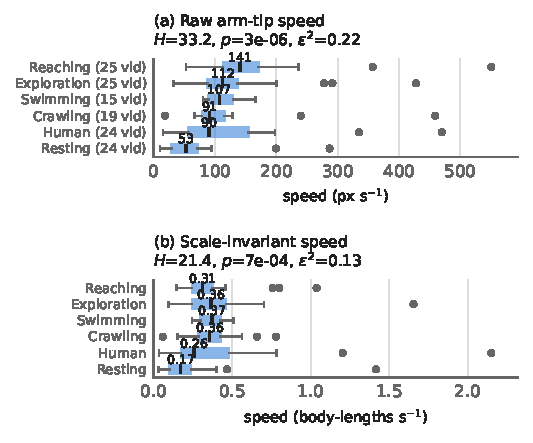
\includegraphics[width=0.47\textwidth]{assets/kinematics_by_behaviour.pdf}
    \caption{State-gated arm-tip speed by VLM-assigned behaviour class ($146$
    clips / $66$ source videos, $\leq\!2$ per video). Each box summarises the
    per-\emph{video} medians---the independent unit, since clip-level pooling
    would be pseudo-replication; dots are videos beyond the whiskers. (b)
    divides speed by arm spread, removing the apparent-size confound; both
    panels keep the class order of (a), so the rank change is visible: reaching
    is fastest in raw pixels but third in body-lengths per second, being
    performed with an extended body.}
    \label{fig:kinematics}
\end{figure}

\textbf{Cross-validation of the two signal paths.} Merging per-clip kinematics
into the structured records gives an independent check on the VLM labels, tested
on a behaviour-stratified sample of $146$ clips from $66$ source videos
($\sim\!25$ clips per class, at most two per video) and aggregated to one value
per (video, class) before any test, since clips from one recording are not
independent. State-gated arm-tip speed separates the classes in the
direction ethology expects (Fig.~\ref{fig:kinematics}): median $53$\,px\,s$^{-1}$
for resting, rising through human interaction, crawling, swimming and
exploration to $141$ for reaching out of water (Kruskal--Wallis $H{=}33.2$,
$p{=}3.5\!\times\!10^{-6}$, $\varepsilon^2{=}0.22$ over $132$ video--class
units; all five resting-vs-class contrasts significant after Holm correction).
Raw pixel speed confounds motion with apparent size, so every test is repeated
on speed divided by arm spread---body-lengths per second---and the separation
survives ($H{=}21.4$, $p{=}6.8\!\times\!10^{-4}$, $\varepsilon^2{=}0.13$, all
five contrasts still significant). The normalised view also corrects the raw
one: reaching is fastest in pixels but only third in body-lengths per second,
being performed with an extended body, while swimming and crawling rise. Since
the two pathways share no components beyond the raw video, their agreement
indicates both track real behaviour rather than each other's artefacts---though
it shows the kinematics follow the labels, not that the labels are correct. The
labels are in fact only moderately self-consistent (Cohen's $\kappa{=}0.55$,
below), which cuts in this result's favour: label noise unrelated to motion
dilutes a group-difference test toward the null, so the separation found here is
likely conservative. An earlier
$n{=}40$-clip version, pooled at clip level, gave the same ordering with more
extreme endpoints ($63$ to $159$\,px\,s$^{-1}$); the powered estimate is the
more conservative one. Speeds are camera-relative pixels; metric calibration is
future work.

\textbf{Relevance to the OCEANS community.} The work targets intelligent sensing
and longitudinal behavioural analysis for controlled marine habitats, and
emphasises \emph{edge deployability}: the students run offline on commodity
hardware, so in-situ monitoring needs no cloud. Where the companion system acts
on one behaviour in real time, this pipeline supplies the baseline against which
such events are interpreted.

\section{Limitations and Ongoing Work}
\label{sec:limits}
We are deliberate about what is not yet established.
\begin{itemize}[leftmargin=*, itemsep=1pt, topsep=2pt]
\item \textbf{Human-verified test sets exist only for segmentation} ($499$ human
masks; five source videos excluded from \emph{all} training sources). Detection
and captioning stay on internal splits, so we make no comparative claims there.
\item \textbf{The behaviour labels are only moderately self-consistent, and every
aggregate result is grouped by them.} Re-annotating a frozen sample of $250$
clips from $140$ recordings with a \emph{disjoint} set of input frames changes
roughly a third of the behaviour labels: raw agreement $0.652$, Cohen's
$\kappa{=}0.552$, CI95 $[0.472,0.624]$---``moderate''. This bounds the activity
budget, circadian profile, stimulus response and kinematics cross-validation
alike. It measures \emph{consistency under frame sampling}, not accuracy: a
perfectly consistent extractor can be consistently wrong, and validation against
a human ethologist remains the larger open item. Noise of this kind, if
independent of motion, attenuates group differences toward the null, so the
kinematics separation (Sec.~\ref{sec:skeleton}) is likely understated rather
than inflated---an argument that fails if fast clips are preferentially
mislabelled, which we cannot yet test. The rare classes are least stable
(swimming/jetting $43\%$ reproduced, $n{=}7$; reaching out of water $48\%$,
$n{=}21$) and are also the classes with the fewest recordings in the kinematics
test, so per-class claims about them deserve extra caution.
\item \textbf{Leakage is easy and we hit it once.} Two label sources sharing
source videos silently placed test videos in training; an apparent
$0.49\!\rightarrow\!0.70$ improvement evaporated under a hard video-level
holdout. All results here post-date that correction and the current holdout was
re-verified (Sec.~\ref{sec:bench}).
\item \textbf{The presence gate is now powered, but not unbiased everywhere.}
The frozen suite's $19$ empty-tank negatives (two recordings) are superseded by
the human-verified multi-recording sets of Table~\ref{tab:presence}; the
reflection subset used for the head-to-head, however, is still drawn from
extractor-selected clips, so that comparison's effect size is an upper bound.
Absolute behavioural rates depend on this gate; we report contrasts, which are
robust to a constant gate bias.
\item \textbf{Mask errors are localisation errors, and the cheap temporal fix
fails.} Body area is accurate to $\sim\!1\%$ while IoU is $0.64$: the mask is the
right size in the wrong place. Test-time fusion does not repair this even at
each variant's best threshold; a temporally \emph{trained} student is untested.
\item \textbf{Context label is coarse.} ``Enrichment interaction'' fires
whenever a permanent tank object is visible ($\sim$66\% of clips); the clean
stimulus contrast is human-present vs.\ absent.
\item \textbf{Skeleton and kinematics.} Arm recovery is silhouette-limited: even
human masks expose only $5.7$ arm protrusions per frame and the model's masks
cost more, so tip recall stands at $0.50$. Kinematics cover a $146$-clip
stratified sample, with swimming/jetting on the fewest recordings ($15$), and
infrared cameras are not covered by the colour-trained segmenter. A
static-feature behaviour classifier failed (below the majority baseline),
confirming that behaviour classification needs temporal features rather than
more labels---which the kinematics layer supplies.
\end{itemize}
Ongoing work: extending the kinematics to the full corpus and validating the
behaviour labels against a human ethologist; distilling the structured extractor
into the local $2$-B student (JSON targets rather than a sentence); and, to pass
the silhouette ceiling, a learned keypoint model on RGB appearance rather than
masks.

\section{Conclusion}
We presented an automated vision--language pipeline that converts continuous
octopus footage into a quantified behavioural and affective-state time-series and
distils its large teachers into local models that run offline. It surfaces an
interpretable activity budget, a circadian rhythm and a measurable stimulus
response; the segmentation student---evaluated leak-free on a human-verified
test---supplies the presence signal and the masks for an anatomical skeleton
whose occlusion-honest kinematics separate the language-model behaviour classes
under video-level statistics. Reported with its negative results and leakage
lessons, it offers a practical, welfare-oriented layer for longitudinal
behavioural understanding in controlled marine habitats.

\section*{Ethical Statement and Data Availability}
The work was conducted in a private aquarium, with only sub-threshold
interactions w.r.t.\ EC directive 2010/63/EU of several caretakers with a single
\emph{O.\ vulgaris} (supplier: Flying Sharks, Portugal). Husbandry and enrichment
followed best practice under FELASA guidelines. Video data are available from
the last author.

\footnotesize
\begin{thebibliography}{00}
\bibitem{disc_o}
K.\ Patel, A.\ Sharma, H.\ Kumar, P.\ Kurundodi, H.\ Burgsteiner, and W.\ Slany,
``A Novel Framework for Decoding Inter-Species Communication with Octopodes
(DISC-O),'' in \textit{OCEANS 2025}, pp.\ 1--9, Sep.\ 2025,
doi: 10.23919/OCEANS59106.2025.11244956.
\bibitem{clip}
A.\ Radford \textit{et al.}, ``Learning Transferable Visual Models from Natural
Language Supervision,'' in \textit{ICML}, 2021.
\bibitem{groundingdino}
S.\ Liu \textit{et al.}, ``Grounding DINO: Marrying DINO with Grounded Pre-Training
for Open-Set Object Detection,'' \textit{arXiv:2303.05499}, 2023.
\bibitem{sam2}
N.\ Ravi \textit{et al.}, ``SAM 2: Segment Anything in Images and Videos,''
\textit{arXiv:2408.00714}, 2024.
\bibitem{lora}
E.\ J.\ Hu \textit{et al.}, ``LoRA: Low-Rank Adaptation of Large Language Models,''
in \textit{ICLR}, 2022.
\bibitem{mobilenetv3}
A.\ Howard \textit{et al.}, ``Searching for MobileNetV3,'' in \textit{ICCV}, 2019.
\bibitem{qwenvl}
Qwen Team, ``Qwen3-VL,'' 2025.
\bibitem{owlv2}
M.\ Minderer, A.\ Gritsenko, and N.\ Houlsby, ``Scaling Open-Vocabulary Object
Detection,'' in \textit{NeurIPS}, 2023.
\bibitem{hideandseg}
A.\ de Aguiar, M.\ P.\ Andrade, C.\ M.\ D.\ Santos, and J.\ P.\ Gois,
``HideAndSeg: an AI-based tool with automated prompting for octopus segmentation
in natural habitats,'' \textit{arXiv:2511.04426}, Nov.\ 2025.
\end{thebibliography}

\end{document}
